\section{系统的结构}

\subsection{直接实现}

\begin{BoxProperty}[通过梅森公式直接实现构造信号流图]*
    将系统函数化为以下形式
    \begin{Equation}
        H(s) = \frac{b_ms^{-(n-m)}+b_{m-1}s^{-(n-m+1)}+\dots+b_0s^{-n}}{1-(-a_{n-1}s^{-1}-a_{n-2}s^{-2}-\dots-a_0s^{-n})}
    \end{Equation}
    其中分子每项为一条前向通路,分母除$1$外每项为一条回路。
    构造可得
    \begin{Figure}[梅森公式直接构造]
        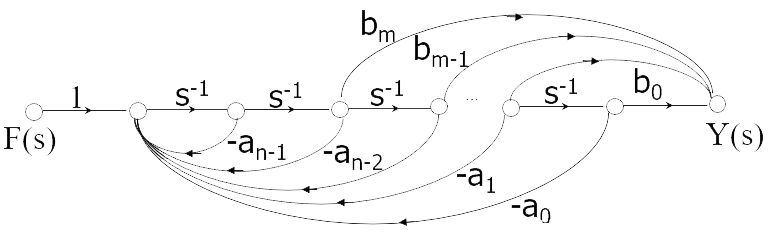
\includegraphics[width=80mm]{img/7.7.png}
    \end{Figure}
\end{BoxProperty}

\subsection{级联实现}

\begin{BoxProperty}[级联实现构造信号流图]*
    将$H$分解为若干一阶或二阶的系统函数的乘积,即
    \begin{Equation}
        H = H_1H_2\dots H_n
    \end{Equation}
    将分解后的系统级联即可。

    其中一阶系统函数形式为
    \begin{Equation}
        H_i(s) = \frac{s+b_0}{s+a_0}
    \end{Equation}
    其中二阶系统函数形式为
    \begin{Equation}
        H_i(s) = \frac{s^2+b_{1i}s+b_{0i}}{s^2+a_{1i}s+a_{0i}}
    \end{Equation}
\end{BoxProperty}

\subsection{并联实现}

\begin{BoxProperty}[并联实现构造信号流图]*
    将$H$展开为部分分式,将每个分式分别作为支路增益,再将各支路并联。

    即将$H$化为以下形式再构造
    \begin{Equation}
        H(s) = \frac{b_0}{s}+\frac{b_1}{s+a_1}+\frac{b_2}{s+a_2}+\dots+\frac{b_n}{s+a_n}
    \end{Equation}
\end{BoxProperty}